\section{Background}
\begin{figure}
\centering
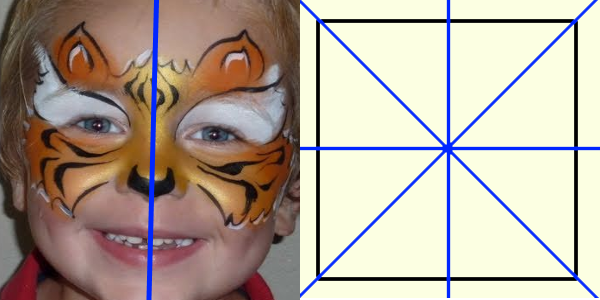
\includegraphics[width=0.9\columnwidth]{reflection}
\caption{On the left, a face, exhibiting bilateral vertical reflection symmetry. On the right, a square, which contains four reflection axes. Reflection axes are marked with blue lines. Notice that mirroring the images about any of the axes would result in the same image}
\label{ref}
\end{figure}

In two-dimensional images, there are only four symmetric transformations that are not a composition of other transformations. These are \textit{reflection}, \textit{rotation}, \textit{glide reflection}, and \textit{translation}. Various combinations of these symmetries are what differentiate the seventeen wallpaper groups. We note that human perception does not necessarily rely on perfect symmetry. While textures which have been manipulated can pose a serious problem for computer vision algorithms, humans are quite good at recognizing patterns even in significantly distorted images \cite{nearregular}.  

Reflection is the most well-known symmetry, with the vernacular for symmetry referring to it exclusively. Objects that contain reflection have a reflection \textit{axis}, a line that separates the image into two mirrored halves. Examples of reflection symmetry in nature include the faces and bodies of animals. Reflection is often characterized by the number of reflection \textit{axes} that can divide the object. A face, for instance, would only contain one. A square, on the other hand, would contain three (see Figure~\ref{ref}).

Rotation symmetry also frequently in nature. Rotation symmetry refers to an object's ability to rotate around some center without changing. It is characterized by the number of rotation angles that maintain this symmetry. For instance, a hexagon and a flower with six pedals would both have 6-fold rotation symmetry (see Figure~\ref{rot}). On the other hand,

\begin{figure}
\centering
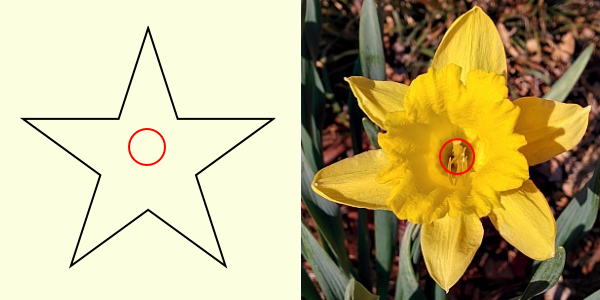
\includegraphics[width=0.9\columnwidth]{rotation}
\caption{On the left, a flower exhibiting 6-fold rotation symmetry. On the right, a six-pointed star, exhibiting 6-fold rotation symmetry. Rotation centers for each are marked with red circles}
\label{rot}
\end{figure}

Translation symmetry is when an object contains repeating \textit{tiles}. Tiles are small identical pieces of the image that repeat. For instance, in a brick wall, a single brick could be the tile. An infinitely long brick wall contains symmetry because shifting every brick to the right by the length of one brick leaves the wall appearing exactly the same. Another example of translation symmetry is a fence. If the fence was shifted by the length from one post to the next, the fence would stay the same. See Figure~\ref{trans} for examples.

\begin{figure}
\centering
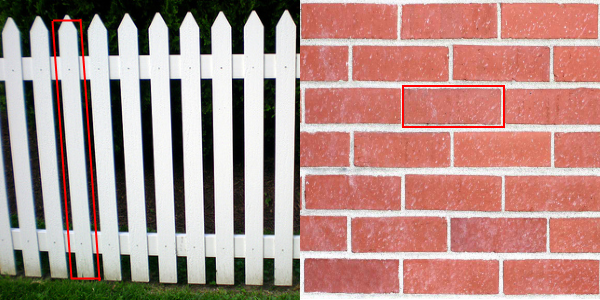
\includegraphics[width=0.9\columnwidth]{translation}
\caption{On the left, a white fence. On the right, a brick wall. In both of these images, the image would have to repeat infinitely to truly exhibit translation symmetry. The tile is outlined in red. In the brick wall, the brick could be shifted along two separate axes, while in the white fence, it would have to be shifted left or right.}
\label{trans}
\end{figure}

The last basic symmetry is glide reflection. Glide reflection requires translation symmetry to exist. While reflection refers to an object directly mirrored across an axis, glide reflection is when the object is mirrored at exactly half of the translation distance. One example of glide reflection in nature are footsteps. Halfway in between each footstep, there is a reflected footstep (made by the other foot). Importantly, it is impossible to have glide reflection and reflection along the same axis. For instance, if two sets of footsteps form exact mirrors of each other, then that axis is said to have reflection, not glide reflection (see Figure~\ref{glide}).

\begin{figure}
\centering
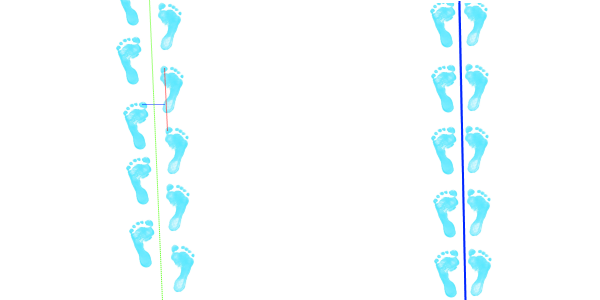
\includegraphics[width=0.9\columnwidth]{glide}
\caption{On the left, footsteps exhibiting a glide reflection pattern. On the right, footsteps exhibiting a normal reflection pattern. Note that along any given axis, only one is possible. If its mirrored after translation, it is glide reflection. If it is mirrored without translation, it is normal reflection.}
\label{glide}
\end{figure}

In the wallpaper groups, every group has translation symmetry and a unique set of other symmetries. The seventeen groups comprise all possible sets. Table~\ref{sym-tab} gives a description of the seventeen groups in terms of their symmetries. Notably, sometimes even when both groups have reflection, they have it along different axes. See Figure~\ref{fig:P4GvP4M} for an example. Importantly, any single group would have the exact same symmetries, even if their appearance was different. See Figure~\ref{P4MvP4M} for an example. Every group also has its own \textit{tile shape}, which is the shape of the smallest repeating piece of the image.

\begin{table}[!ht]
\centering
\resizebox{\columnwidth}{!}{%
\begin{tabular}{|l|c|c|c|c|c|c|c|c|c|}
\hline
Group & 2-fold & 3-fold & 4-fold & 6-fold & $T_1$ & $T_2$ & $D_1$ & $D_2$ &  tile \\ \hline
P1 & F & F & F & F & None & None & None & None & O \\ \hline
P2 & T & F & F & F & None & None & None & None & O \\ \hline
PM & F & F & F & F & Refl & None & None & None & Re \\ \hline
PG & F & F & F & F & Glide & None & None & None & Re \\ \hline
CM & F & F & F & F & None & None & Refl & None & Rh \\ \hline
PMM & T & F & F & F & Glide & Refl & None & None & Re \\ \hline
PMG & T & F & F & F & Glide & Refl & None & None & Re \\ \hline
PGG & T & F & F & F & Glide & Glide & None & None & Re \\ \hline
CMM & T & F & F & F & None & None & Refl & Refl & Rh \\ \hline
P4 & T & F & T & F & None & None& None & None & S \\ \hline
P4M & T & F & T & F & Refl & Refl & Refl & Refl & S \\ \hline
P4G & T & F & T & F & Glide & Glide & Refl & Refl & S \\ \hline
P3 & F & T & F & F & None & None & None & None & H \\ \hline
P3M1 & F & T & F & F & None & None & Refl& None & H \\ \hline
P31M & F & T & F & F & Refl & Refl & Refl & None & H \\ \hline
P6 & T & T & F & T & Refl & None & None & None & H \\ \hline
P6M & T & T & F & T & Refl & Refl & Refl & Refl & H \\ \hline
\end{tabular}%
}
\caption{Wallpaper groups represented as their symmetries. The first four columns are whether the group has that type of rotation symmetry. The second four columns refer to the four main axes on the tile. (Refl=Reflection, Glide=Glide Reflection, Re=Rectangular, Rh=Rhombic, O=Oblique, S=Square, H=Hexagonal)}
\label{sym-tab}
\end{table}

In representing wallpaper groups as a set of symmetries, we can form relationships among the groups based on these sets. Every group's symmetries are either a subset or a superset of every other group. If each group is placed with its relation to other groups, they form a graph, see Figure~\ref{graph}. Note that replacing glide reflection with reflection along an axis maintains the superset relationship. See Table~\ref{sym-tab} to otherwise see that this hierarchy is formed. Note that the tile shape is not part of the group-theoretic analysis.

\begin{figure}[!ht]
\centering
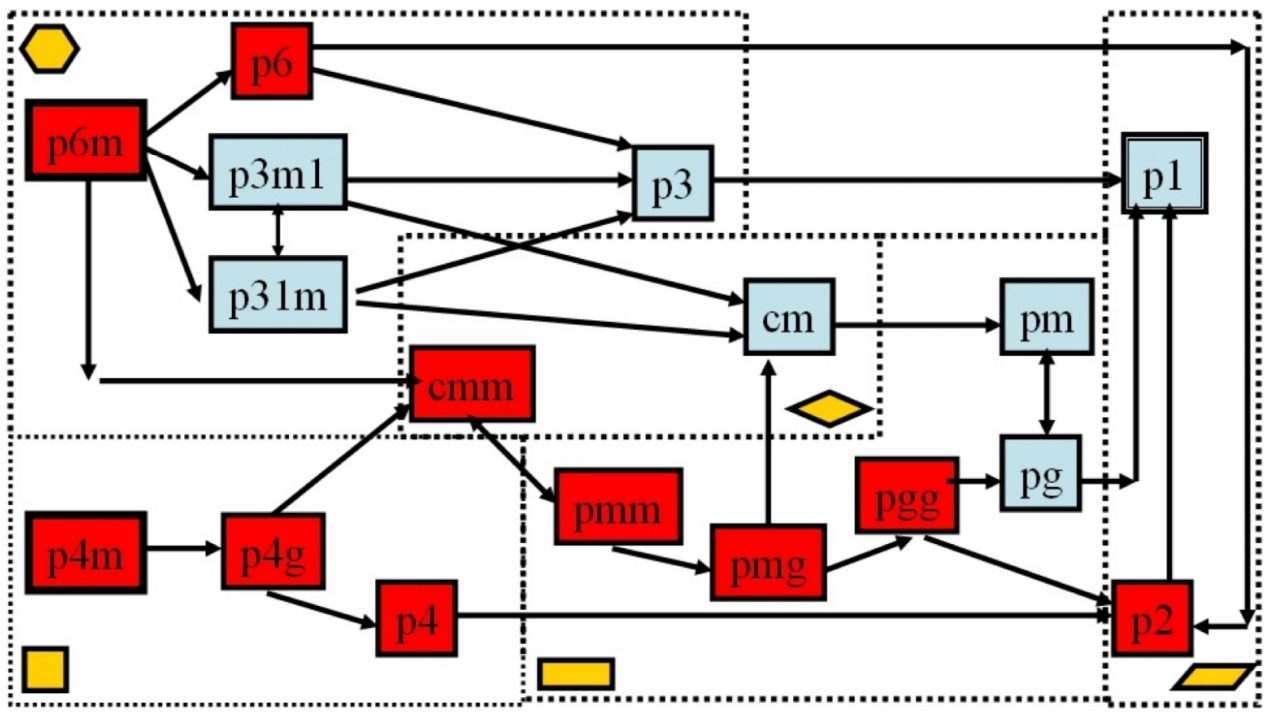
\includegraphics[width=0.9\columnwidth]{Yanxi_Graph}
\caption{The subgroup relation graph. If an arrow points from any given box, $A$, toward any given box $B$, that means that $B$'s symmetries are subset of $A$'s symmetries.}
\label{graph}
\end{figure}